\documentclass{book}
\usepackage[T1]{fontenc}
\usepackage{graphicx}
\usepackage{amsmath}
%\usepackage{pdflscape}
%\usepackage{afterpage}
%\usepackage{changepage}
%\usepackage{caption}
%\usepackage{rotating} %for sidewisetable
%\usepackage{makecell}
%\usepackage{boldline}

% włączenie polskich znaków
\usepackage[english]{babel}
\usepackage{hyperref}
\usepackage{color}
\usepackage{framed}
\usepackage{listings}
\usepackage[most]{tcolorbox}
\usepackage{filecontents}
\usepackage{tabularx}


\newenvironment{header}{\bgroup\Large}{\egroup}

\newenvironment{code2}{
    \par\medskip
    \begin{framed}
    \noindent\ignorespaces
}
{
    \end{framed}
    \medskip
}

\newenvironment{explain}{
    \par\medskip
    \begin{framed}
    \noindent\ignorespaces
}
{
    \end{framed}
    \medskip
}

\newenvironment{extercises}{
    \par\medskip
    \begin{framed}
    \noindent\ignorespaces
}
{
    \end{framed}
    \medskip
}


\definecolor{maroon}{rgb}{0.5,0,0}
\definecolor{DarkOliveGreen}{rgb}{0.33,0.42,0.18}
\definecolor{darkgreen}{rgb}{0,0.5,0}

\lstdefinelanguage{XML}
{
  basicstyle=\ttfamily\footnotesize,
  morestring=[b]",
  moredelim=[s][\bfseries\color{maroon}]{<}{\ },
  moredelim=[s][\bfseries\color{maroon}]{</}{>},
  moredelim=[l][\bfseries\color{maroon}]{/>},
  moredelim=[l][\bfseries\color{maroon}]{>},
  morecomment=[s]{<?}{?>},
  morecomment=[s]{<!--}{-->},
  commentstyle=\color{DarkOliveGreen},
  stringstyle=\color{blue},
  identifierstyle=\color{red}
}

\lstdefinelanguage{JavaScript}{
  keywords={break, case, catch, continue, debugger, default, delete, do, else, false, finally, for, function, if, in, instanceof, new, null, return, switch, this, throw, true, try, typeof, var, void, while, with},
  morecomment=[l]{//},
  morecomment=[s]{/*}{*/},
  morestring=[b]',
  morestring=[b]",
  ndkeywords={class, export, boolean, throw, implements, import, this},
  keywordstyle=\color{blue}\bfseries,
  ndkeywordstyle=\color{darkgray}\bfseries,
  identifierstyle=\color{black},
  commentstyle=\color{purple}\ttfamily,
  stringstyle=\color{red}\ttfamily,
  sensitive=true
}


\newtcblisting{html}[1][]{
  listing only,
  breakable,
  colframe=cyan,
  colback=cyan!10,
  %title=#1,
  listing options={
    language=XML,
    basicstyle=\small\ttfamily,
    breaklines=true,
    columns=fullflexible
  },
  #1
}

\newtcbinputlisting{\htmlfile}[3][]{
  listing only,
  breakable,
  colframe=cyan,
  colback=cyan!10,
  %title=#1,
  left=6mm,
  listing options={
    language=XML,
    basicstyle=\small\ttfamily,
    breaklines=true,
    columns=fullflexible,
    numbers=left,numberstyle=\tiny\color{red!75!black}
  },
  listing file=#2
}

\newtcblisting{js}[1][]{
  listing only,
  breakable,
  colframe=cyan,
  colback=cyan!10,
  %title=#1,
  listing options={
    language=JavaScript,
    basicstyle=\small\ttfamily,
    breaklines=true,
    columns=fullflexible,
  },
  #1
}

\newtcbinputlisting{\jsfile}[3][]{%
  listing only,
  breakable,
  colframe=cyan,
  colback=cyan!10,
  left=6mm,
  %title=#1,
  listing options={
    language=JavaScript,
    basicstyle=\small\ttfamily,
    breaklines=true,
    columns=fullflexible,
    numbers=left,numberstyle=\tiny\color{red!75!black},
    #1
  },
  listing file=#2
}

\newtcbinputlisting{\phpfile}[3][]{%
  listing only,
  breakable,
  colframe=cyan,
  colback=cyan!10,
  left=6mm,
  %title=#1,
  listing options={
    language=PHP,
    basicstyle=\small\ttfamily,
    breaklines=true,
    columns=fullflexible,
    #1
  },
  listing file=#2
}

\newtcblisting{shell}[1][]{
  listing only,
  breakable,
  colframe=cyan,
  colback=black,
  colupper=white,
  %title=#1,
  every listing line={\textcolor{red}{\small\ttfamily\bfseries \$> }},
  listing options={
    language=sh,
    basicstyle=\small\ttfamily,
    breaklines=true,
    columns=fullflexible
  },
  #1
}

\newtcbinputlisting{\bashfile}[3][]{%
  listing only,
  breakable,
  colframe=cyan,
  colback=black,
  colupper=white,
  %title=#1,
  listing options={
    language=sh,
    basicstyle=\small\ttfamily,
    breaklines=true,
    columns=fullflexible,
    #1
  },
  listing file=#2
}

\newenvironment{warning}{\bgroup \color{red} }{\egroup}

\newenvironment{remark}{
    \par\medskip
    \begin{framed}
    \noindent\ignorespaces
}
{
    \end{framed}
    \medskip
}

\begin{document}
\chapter{Introduction to jQuery }

Before we start with Mobile Application development let us first introduce a very well known and useful library jQuery. Here we will cover some basics of jQuery library and how to use it for simple internet queries. The jQuery library basically can be used to do following operations:
\begin{itemize}
\item Manipulation of HTML/DOM elements in a web application.
\item Manipulation of CSS properties/elements in a web application.
\item Operations connected to HTML events.
\item Simple effects and animations in a web application.
\item AJAX operations.
\end{itemize}



\section{Include jQuery into a project}
The jQuery can be included int our project in two simple ways:
\begin{itemize}
\item As external resource,
\item As internal resource,
\end{itemize}

The difference is only on loading time and requirements of available internet connectivity.
\begin{html}
<!-- Use External jQuery from Google CDN -->
<script type="text/javascript"
    src="https://ajax.googleapis.com/ajax/libs/jquery/3.3.1/jquery.min.js">
</script>
<!-- Use External jQuery from Microsoft CDN -->
<script type="text/javascript"
    src="https://ajax.aspnetcdn.com/ajax/jQuery/jquery-3.3.1.min.js">
</script>
<!-- Use Internal copy of jQuery library -->
<script type="text/javascript"
    src="js/jquery-3.3.1.min.js">
</script>
\end{html}
As for Cordova javascript elements we will put one of this at the end of <body> section of web page. At this moment 3.3.1 is the newest version of jQuery, however everybody can use the version of own choose. The library files are usually available in two versions jquery-3.3.1.js and jquery-3.3.1.min.js, the former is bigger and is made especially for developers to analyse while the latter is smaller and unreadable for people because all unneeded space characters are omitted, this version is preferred as it requires shorter time to load and smaller bandwidth.

\section{Selector operator}
One of the most important element introduced in jQUery is selection operator \$, this is an shortcut to original javascript selection methods like getElementById or querySelector.

\jsfile{chapters/code_samples/chapter_jquery_intro/code1.js}

With use of selector we can easily operate on DOM elements of our web pages. DOM - Document Object Model - an object representation of html document and its elements. However, we have to remember jQuery selector is not exactly document.getElementById operation, by default selector wraps all elements that fits the pattern so it is more like the list of appropriate objects than a single object. That means selector has no direct access to all object methods. In order to get a DOM object from selector we should use direct request of list element like in the following code:

\begin{js}
var el = document.getElementById("some_id");
//Equivalent operation with use of jQuery selector
var el = $("#some_id")[0];
\end{js}


\section{Add simple actions when page is load}
When a selector gives an object we can bind operations to events connected with this object. For example object "document" - that represents the web page have an event onLoad. This event is fired whenever  the browser finish loading page with all required additional files.

\htmlfile{chapters/code_samples/chapter_jquery_intro/code2.html}

\begin{explain}
Just for simplicity this time all js code was simply included inside .html file. In the line 10 we can see selector \$('document') and then an definition what should happen when page is 'ready' event is fired.
\begin{js}
	$(document).ready(
\end{js}

Inside "ready(...)" we define a new anonymous function that will be bind to 'ready' event. The function is anonymous as it is a method that will be used in one place and no name is needed. Anonymous functions are usually defined as:
\begin{js}
 function() { ...} //anonymous function without parameters
 function(par1, par2) { ...} //anonymous function with two parameters par1 and par2
\end{js}

In this new function in the line 13 we can see that to all <button> elements we add a function that hides this button. An operation .hide comes from jQuery and allow to make elements invisible.

\begin{js}
$("button").click(function(){
    $(this).hide();
});
\end{js}

In the result when page is loaded the actions are added to all three buttons separately. When each of the buttons is clicked it hides.


\end{explain}

It it obvious that if in jQuery we have hide operation, there have to be also a show one

\htmlfile{chapters/code_samples/chapter_jquery_intro/code3.html}

\begin{explain}
We add anonymous function to click event for both buttons "btn1" and "btn2" in the lines 15 and 19 respectively. in both of this methods we show or hide the element <img>.
\end{explain}

\begin{extercises}
Starting with the webpage of the form

\htmlfile{chapters/code_samples/chapter_jquery_intro/ex1.html}

Add the following functionalities:
\begin{itemize}
\item When user click on the button "Show Julius Caesar" the photo of the Caesar is shown
\item When user click on the button "Show All" every hidden elements are shown
\item When user click on the button "Hide all again" all elements back to the original state.
\end{itemize}
\end{extercises}

In the next example we will see that a similar jQuery method called toggle, can be used show the visible elements and hide invisible ones.

\htmlfile{chapters/code_samples/chapter_jquery_intro/code4.html}

\begin{explain}
At the start one of the <p> elements is hidden as in line 14  we set style to display:none state.
\begin{html}
<p id="Stanza2" style="display:none">
\end{html}
Here in the line 27 we invoke toggle method on all <p> element. This will toggle elements between two states hidden and shown.
\end{explain}

Additional jQuery actions like slideDown, slideUp, slideToggle allows similar operations but as animated action not instant ones.

\htmlfile{chapters/code_samples/chapter_jquery_intro/code5.html}

\begin{extercises}
Within the last code change methods slideDown, slideUp, slideToggle into new operations: fadeIn, fadeOut, fadeToggle.
\end{extercises}

\begin{extercises}
All of the animation operations can have additional time parameters (in milliseconds), test how it changes the original behaviour.
\begin{js}
.hide(300),
.slideDown(300),
.fadeOut(300)
\end{js}


There are also predefined speeds 'slow', 'fast', 'normal':
\begin{js}
.show('fast')
\end{js}
\end{extercises}

\subsection{Other actions}
jQuery introduces more operations like click, these are dblclick, mouseover, mouseout. And additionally more sophisticated animation driven by changes in the style of the element

\htmlfile{chapters/code_samples/chapter_jquery_intro/code6.html}

\begin{explain}
  As we can see during animate operation the browser create an animation between two styles
  \begin{js}
    width: "55%",
    opacity: 0.7,
    fontSize: "2em",
  \end{js}
   and
  \begin{js}
    fontSize: "1em",
  \end{js}

This animation requires change of width, size of the font and opacity.
\end{explain} 
\chapter{AJAX queries using jQuery }

Now let us work on AJAX requests using jQuery. The AJAX is an abbreviation for \textbf{A}synchronous \textbf{J}avascript \textbf{A}nd \textbf{X}ml. This technology allows to send (and receive) information from external sources via asynchronous queries. Usually the data send back and forth is in JSON (\textbf{J}ava\textbf{S}cript \textbf{O}bject \textbf{N}otation) form. In most of the situations webpages using javascript operations send queries to so called REST services.

\section{RESTful services}
As usual nowadays most of internet services provide so called REST services. This type of services allows us to invoke basic CRUD operations (\textbf{C}reate, \textbf{R}ead, \textbf{U}pdate, \textbf{D}elete). REST API usually allows 4 basic types of http queries GET, POST, PUT and DELETE on so called resources. These operations are usually connected with operations on the resources identified by url. For example GET is a Read or show the resource, POST and PUT are Create or Update the resource, meaning of DELETE is obvious. There is no canonical way for distinction of two operations POST and PUT (i.e. every API developer defines when POST or PUT should be used). I suggest to use POST as Create and PUT as Update.

\subsection{Service implementation}
Usually to build a REST client one needs a REST API - service that provides some set of REST operations. The server part can be created in most of server technologies starting with PHP, python, Java, ASP.Net, etc. In this tutorial we will use very simple API created in PHP that can receive and send simple data about user scores in a game.

Here we have sample documentation of our test API service:

\begin{tabularx}{\textwidth}{|l|X|}
\hline
&\textbf{Get selected record}\\\hline
URL &   \url{http://geniusgamedev.eu/cordova/rest_api/rest_srv/:id} or \url{http://geniusgamedev.eu/cordova/rest_api/rest.php?id=:id}\\\hline
Method  & GET\\\hline
Parameters  & id - id of the record \\\hline
Request Data & None\\\hline
Response Data & record object:\\
&
%\begin{js}
\{"data":\{
    "id":2,
    "name":"Helena",
    "score":128
    \}
\}
%\end{js}
\\\hline
\end{tabularx}

\begin{tabularx}{\textwidth}{|l|X|}
\hline
&\textbf{Get all records}\\\hline
URL &   \url{http://geniusgamedev.eu/cordova/rest_api/rest_srv} or \url{http://geniusgamedev.eu/cordova/rest_api/rest.php}\\\hline
Method  & GET\\\hline
Parameters  & None \\\hline
Request Data & None\\\hline
Response Data & record object:\\
&
%\begin{js}
\{"data":\{\\
&"1":\{"id":1,"name":"Alan","score":35\},\\
&"2":\{"id":2,"name":"Helena","score":128\},\\
&"3":\{"id":3,"name":"Alex","score":162\}\\
&\}
%\end{js}
\\\hline
\end{tabularx}

\begin{tabularx}{\textwidth}{|l|X|}
\hline
&\textbf{Add new record}\\\hline
URL &   \url{http://geniusgamedev.eu/cordova/rest_api/rest_srv} or \url{http://geniusgamedev.eu/cordova/rest_api/rest.php}\\\hline
Method  & POST\\\hline
Parameters  & None \\\hline
Request Data & new record object\\
&\{
"data": \{
"id": 1,
"name": "Jane",
"score": 332
\}
\}
\\\hline
Response Data & record object:\\
&
%\begin{js}
\{"data":\{
    "id":12,
    "name":"Jane",
    "score":332
    \}
\}
%\end{js}
\\
&the value id is a new value created by the service
\\\hline
\end{tabularx}

\begin{tabularx}{\textwidth}{|l|X|}
\hline
&\textbf{Update a record}\\\hline
URL &   \url{http://geniusgamedev.eu/cordova/rest_api/rest_srv/:id} or \url{http://geniusgamedev.eu/cordova/rest_api/rest.php?id=:id}\\\hline
Method  & PUT\\\hline
Parameters  & id - id of the record tu update \\\hline
Request Data & new record object\\
&\{
"data": \{
"id": 1,
"name": "Jane",
"score": 332
\}
\}
\\\hline
Response Data & record object:\\
&
%\begin{js}
\{"data":\{
    "id":3,
    "name":"Jane",
    "score":332
    \}
\}
%\end{js}
\\
&the value id is an id of updated record
\\\hline
\end{tabularx}

\begin{tabularx}{\textwidth}{|l|X|}
\hline
&\textbf{Delete selected record}\\\hline
URL &   \url{http://geniusgamedev.eu/cordova/rest_api/rest_srv/:id} or \url{http://geniusgamedev.eu/cordova/rest_api/rest.php?id=:id}\\\hline
Method  & DELETE\\\hline
Parameters  & None \\\hline
Request Data & None\\\hline
Response Data & record object:\\
&
%\begin{js}
\{"data":\{\\
&"1":\{"id":1,"name":"Alan","score":35\},\\
&"3":\{"id":3,"name":"Alex","score":162\}\\
&\}
%\end{js}
\\
&the rest of records after erasing the requested element
\\\hline
\end{tabularx}

% GET http://geniusgamedev.eu/cordova/rest_api/rest_srv/1
% POST http://geniusgamedev.eu/cordova/rest_api/rest_srv/1

In order to test first two of presented operations we can in the browser open one of these two addresses: \url{http://geniusgamedev.eu/cordova/rest_api/rest_srv} \url{http://geniusgamedev.eu/cordova/rest_api/rest_srv/2}.

\subsection{Prepare page for our rest client}
At first let us create base for our web rest client.

\htmlfile{chapters/code_samples/chapter_jquery_ajax/code1.html}

and starting js file

\jsfile{chapters/code_samples/chapter_jquery_ajax/code1.js}

\begin{explain}
As we can see in html file we have a <table id="result\_tbl"> where results obtained from service will be placed. Additionally we have appropriate buttons for GET, POST and PUT operations. Now we just need to fill the methods getOneRecord(), getAllRecords(), postRecord(), putRecord(), deleteRecord().
\end{explain}

Firs let us create a simple get query and show the result in alert window:

\begin{js}
function getOneRecord(){
	record_id = 1;
	if ($('#rid').val()) {
		record_id = $('#rid').val();
	}
	$.ajax({
        method : "GET",
        dataType: 'json',
        url: "http://geniusgamedev.eu/cordova/rest_api/rest_srv/"+record_id,
        cache: false
        })
	.done(function (resp) {
		alert(JSON.stringify(resp));
	})
    .fail(function (msg){
      alert(JSON.stringify(msg));
      });
}\end{js}

When this code is inserted into code1.js and the code1.html is run in the browser, we observe that after clicking on the button "getOne\_btn" in the return an alert window with the expected json appears. Changing the value in input field "rid" we change what record will be obtained from the server.

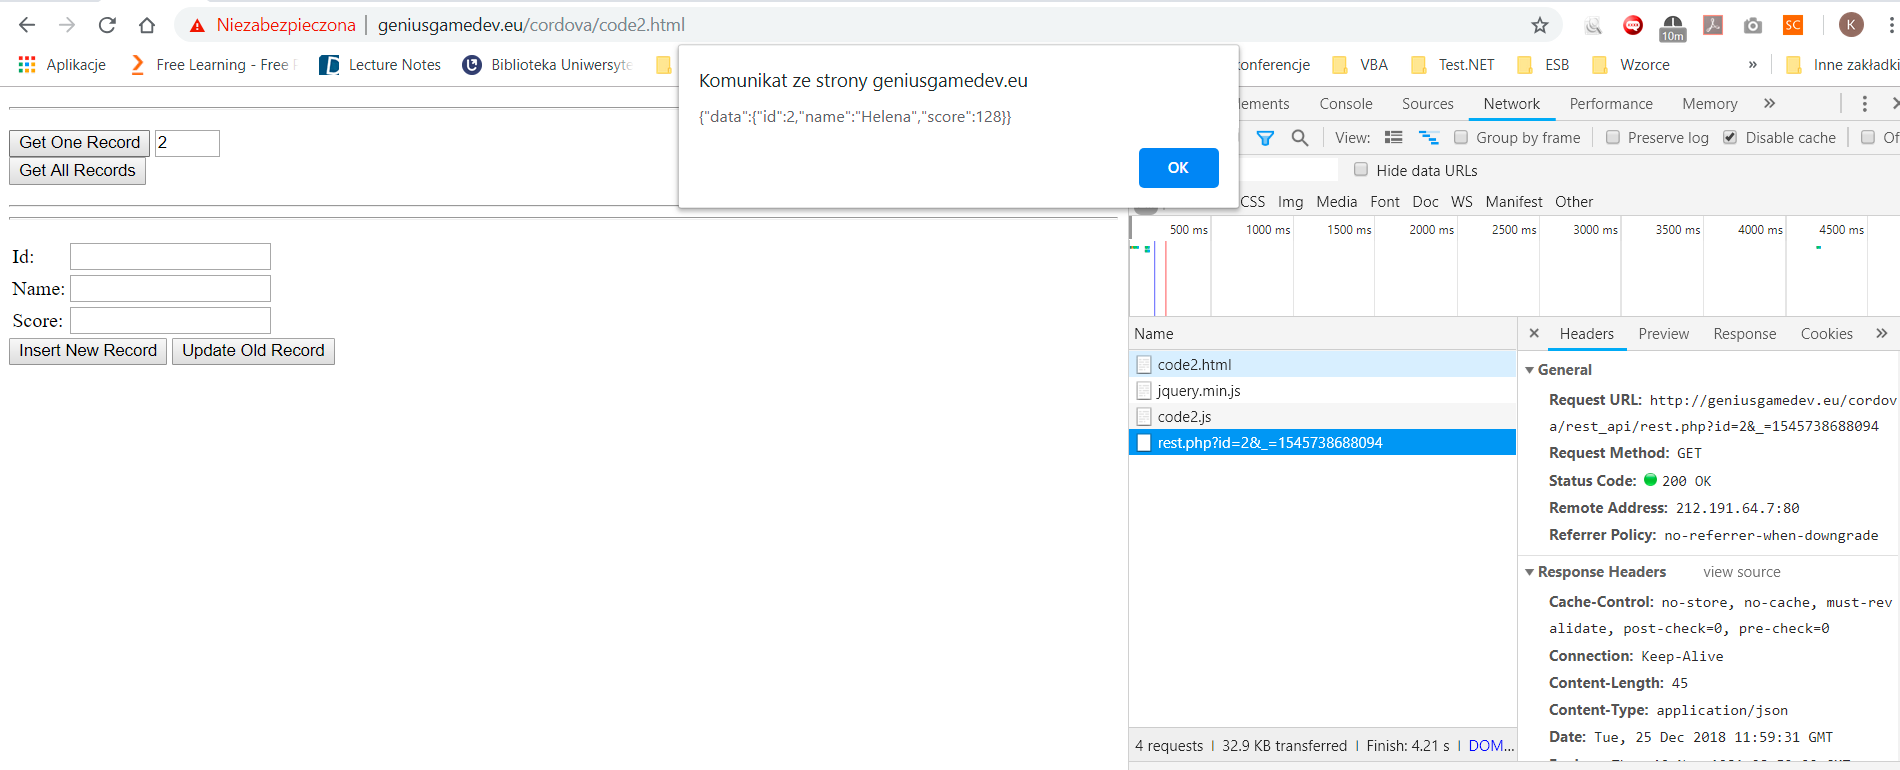
\includegraphics[width=\textwidth]{chapters/img/ajax_screen1.png}

\begin{explain}
In the code w see an operation \$.ajax - this is a shortcut for an AJAX query to the server. This operation has an event "done" that is fired when server respond without errors and "fail" whenever error occurs.
Additionally any json object can be turned into a string using JSON.stringify(). Additionally we see that we are not interested in all response object bun only field data inside this object.
\end{explain}

Now as we know how to obtain an information from server we should work how to add this obtained record into table with results. For that we declare a new function add\_record\_to\_table(record).

\begin{js}
function getOneRecord(){
	record_id = 1;
	if ($('#rid').val()) {
		record_id = $('#rid').val();
	}
	$.ajax({
        method : "GET",
        dataType: 'json',
        url: "http://geniusgamedev.eu/cordova/rest_api/rest_srv/"+record_id,
        cache: false
        })
	.done(function (response) {
		add_record_to_table(response.data);
	})
    .fail(function (msg){
      alert(JSON.stringify(msg));
      });
}

\end{js}

Now we have to create function add\_record\_to\_table(). In that moment we should also think how we should design what element we want to delete. It will be very nice if in every row of our table we will have a DELETE button that will designate record to erasure.

\begin{js}
function add_record_to_table(data){
	var table = $("#result_tbl");
	var new_row = $("<tr/>");
	var cell = $("<td/>");
	cell.html(data.id);
	cell.appendTo(new_row);
	cell = $("<td/>");
	cell.html(data.name);
	cell.appendTo(new_row);
	cell = $("<td/>");
	cell.html(data.score);
	cell.appendTo(new_row);
	cell = $("<td/>");
	var btn = $("<button/>");
	btn.html("DELETE");
	btn.appendTo(cell);
	cell.appendTo(new_row);
	new_row.appendTo(table);
	btn.click(function (){
		deleteRecord(data.id, new_row);
	});
}
\end{js}

\begin{explain}
In order to add a new row in our table we create a new\_row object and each cell for 'id', 'name', 'score' and delete button separately, and append each new cell to a new\_row object. After that we append the new\_row object to existing table and bind a new anonymous function to created button. During erasure we will need id of record to delete from server and the row to get rid off.
\end{explain}

The method deleteRecord can have the form:

\begin{js}
function deleteRecord(record_id, row_to_delete){
	$.ajax({
        method : "DELETE",
        dataType: 'json',
        url: "http://geniusgamedev.eu/cordova/rest_api/rest_srv/"+record_id,
        cache: false
    })
    .done(function (response) {
      row_to_delete.remove();
    })
    .fail(function (msg){
      alert(JSON.stringify(msg));
    });
}
\end{js}

\begin{explain}
  As we can see in jQuery GET and DELETE operations have very similar form. The most important difference is the field 'method'.  Additionally if we want to remove element from our web page it is enough to invoke method .remove() on selected element.
\end{explain}

We already know how to obtain one element via GET operation, the action to get All of them in one query is very straight forward:

\begin{js}
function getAllRecords(){
	$.ajax({
        method : "GET",
		dataType: 'json',
        url: "http://geniusgamedev.eu/cordova/rest_api/rest_srv/",
        cache: false
    })
		.done(function (response) {
			var data = response.data;
			for (let index in data){
				add_record_to_table(data[index]);
			}
		})
		.fail(function (msg){
			alert(JSON.stringify(msg));
		});
}
\end{js}

We are left only with two types of queries "POST" and "PUT", let us start with the first one.

\begin{js}
function postRecord(){
	var new_element = {};
	new_element.id = $("#nid").val();
	new_element.name = $("#name").val();
	new_element.score = $("#score").val();
	var data_to_send ={};
	data_to_send.data = new_element;
	$.ajax({
        method : "POST",
		dataType: 'json',
		data: JSON.stringify(data_to_send),
        url: "http://geniusgamedev.eu/cordova/rest_api/rest_srv/",
        cache: false
    })
		.done(function (response) {
			add_record_to_table(response.data);
		})
		.fail(function (msg){
			alert(JSON.stringify(msg));
		});
}
\end{js}

\begin{explain}
  In the code above at the beginning we have to obtain elements from the form inputs. After that we send the data to server and add a new row from record obtained back. The only new element in this code is setting 'data' field of ajax query.
\end{explain}

The PUT ajax query is very similar to the ones we have already created. And the last piece of the code is an easy extension from previous elements. The final version of js file have the form:

\jsfile{chapters/code_samples/chapter_jquery_ajax/code2.js}



\begin{extercises}
  Please try to make the web page work more efficiently, at the moment if you click 'Get All Records' twice in the table we have doubled every record. Additionally when downloading records one by one we the records in table are not sorted by any means and can repeat.  When asking of a non existing record we obtain error -  as we do not check if reply from the server is not null.
\end{extercises}

 \subsection{Server code}
 The php is not a part of this course, however we have used an exemplary REST server. In order to run appended scripts one have to install WWW server. This examples were tested on Apache server on linux machine and XAMPP installation on Windows 10. The server contains only two files: score.php - connected to database CRUD operations and rest.php - operates on http REST requests.

 \phpfile{chapters/code_samples/chapter_jquery_ajax/score.php}

 \phpfile{chapters/code_samples/chapter_jquery_ajax/rest.php}

 Additionally in order to make this examples run we have to add .htaccess file with the following content:

 \shellfile{chapters/code_samples/chapter_jquery_ajax/.htaccess}

 These files allow simple REST operations using SQLite database \url{http://geniusgamedev.eu/cordova/rest_api/rest/db/score.db}




\chapter{Apache Cordova}

The \href{https://cordova.apache.org}{Apache Cordova} is one of the best known technologies to create modern cross-platform mobile applications. This framework allows to create applications using standard HTML5 technologies stack in order to build mobile apps for Android and iOS mobile devices. The requirements for developer is the knowledge of classical technologies like html, css and JavaScript.

In order to begin work with Cordova environment we have to install \href{http://nodejs.org}{Node.js} application. \begin{warning} This will require administrator privileges on the system.\end{warning} The Node.js environment contains npm - nodejs packet manager that allow to install new packages/application into our system. Using npm we can easily install Cordova by writing in command line:

\begin{shell}
npm install -g cordova
\end{shell}

This -g switch will install cordova for all users, if one wants to install Cordova only for active user we can omit -g parameter.

Now we are ready to create first Cordova app, for that let us create a new directory somewhere in the system and go into this folder.

\begin{shell}
mkdir CordovaApps
cd CordovaApps
\end{shell}

Now we should invoke command:
\begin{shell}
cordova create FirstCordovaApp
\end{shell}

This will create an folder with prepared template of Cordova application. The prepared folder contain few subfolders the most important from the point of view of game developer is www. The rest of subfolders we can treat as internal Cordova folder and let them be.

Just for start we can try to run the project, first we have to add a platform - i.e. the platform we would like to use as deployment machine. In Cordova we have many platforms to choose in this course we will use only Browser for first level debugging, and Android or iOS for second level debugging and final deployment.

\begin{shell}
cd FirstCordovaApp
cordova platform add browser
\end{shell}

And run the created simple starting project

\begin{shell}
cordova run browser
\end{shell}

We should see some information in the terminal and our default browser should open an address \url{http:\\localhost:8000/index.html}. We will see simple page with Cordova logo and a text: device is ready.

Now let us look what is a content of www folder and what lines in the code makes the browser to show this screen \ref{fig.basic_app}.

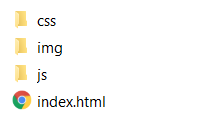
\includegraphics[width=60pt]{chapters/img/basic_structure.png}

We can see specific folders for css, img and js files respectively and one file index.html.

When we open index.html file we will notice the main two parts contained in <head> and <body> tags. At the moment let us ignore <head> part as there is not too many interesting elements and focus on <body>

\begin{html}
<body>
        <div class="app">
            <h1>Apache Cordova</h1>
            <div id="deviceready" class="blink">
                <p class="event listening">Connecting to Device</p>
                <p class="event received">Device is Ready</p>
            </div>
        </div>
        <script type="text/javascript" src="cordova.js"></script>
        <script type="text/javascript" src="js/index.js"></script>
</body>
\end{html}

W can notice few things:
\begin{explain}
\begin{itemize}
\item The JavaScript files are added at the end of the <body> part. This is connected with the order of loading elements in html, and as .js files can operate on html elements it is better to first build these elements before start actions programmed in .js files.

\item We should remember that \begin{warning}cordova.js\end{warning} has to be always the firs script

\item All elements of the web page are contained in one <div class="app"> element

\item There is one <div> element  with id = "deviceready"
\item One <p> element has class listening while the other received

\end{itemize}
\end{explain}

Let us now look into js/index.js file

\jsfile{chapters/code_samples/chapter_cordova_intro/code3.js}

\begin{explain}
How it works: when the page is finally loaded the Cordova environment fire an event 'deviceready', this implies that binded method onDeviceReady is invoked. In the result the method receivedEvent is started with appropriate value of parameter id. In this method the elements with class "listening" becomes invisible while the one with "received" becomes visible.

Explanation line by line:
\begin{description}
\item{line 3:} As we can see in the line 3 the method onDeviceReady is binded to the event 'deviceready'.
\item{line 7:} Run method receivedEvent with parameter id = 'deviceready'
\item{line 11:} Find in the html document the element with id = 'deviceready', store it as parentElement
\item{line 12:} Find all child nodes of parentElement the ones with class "listening", store it as listeningElement
\item{line 13:} Find all child nodes of parentElement the ones with class "received", store it as receivingElement
\item{line 15:} Set style of element listeningElement to display:none, i.e. hide if it is visible on the screen
\item{line 16:} Set style of element receivedElement to display:block, i.e. show if it is not visible on the screen
\item(line 18:) Print a debugging information to JavaScript console.
\item{line 22:} The function initialize of the object app is invoked when javascript is loaded.
\end{description}
\end{explain}

As was mentioned Cordova environment uses a special event 'deviceready'. By default Cordova has more specially defined events, some of them works for all platforms some only for Android (see \url{https://cordova.apache.org/docs/en/latest/cordova/events/events.html}):

\begin{tabularx}{\textwidth}{lX}
'deviceready':& The deviceready event fires when Cordova is fully loaded.\\
'pause': & The pause event fires when the native platform puts the application into the background.\\
'resume':& The resume event fires when the native platform pulls the application out from the background.\\
'backbutton':& The event fires when the user presses the back button.\\
'menubutton':& The event fires when the user presses the menu button. \\
'searchbutton':& The event fires when the user presses the search button on Android. \\
'volumedownbutton':& The event fires when the user presses the volume down button.\\
'volumeupbutton':& The event fires when the user presses the volume up button.\\
\end{tabularx}





\chapter{Cordova and JavaScript games}\label{CordovaAndJavaScriptGame}

You have already learned about JavaScript games in browser and Cordova environment. Cordova allows to run html/css and js code on mobile devices. In this module we will cover how to use the basic game code from previous modules within Cordova environment. In this module we will take one of Canvas basic JavaScript game and run this inside Cordova. As the starting point we take the \href{http://geniusgamedev.eu/canvas/canvas/exampleCode/maze_game.html}{Maze Game example}. This example contains a few files: maze\_game.html, and a set of js, css and png files. At the start let's create basic Cordova project (as was described in previous section). After that combine cordova index.html file with maze\_game.html. Beginning with <head> section of both files we join them into one code:

\begin{html}
<head>
        <meta http-equiv="Content-Security-Policy" content="default-src 'self' data: gap: https://ssl.gstatic.com 'unsafe-eval'; style-src 'self' 'unsafe-inline'; media-src *; img-src 'self' data: content:;">
        <meta name="format-detection" content="telephone=no">
        <meta name="msapplication-tap-highlight" content="no">
        <meta name="viewport" content="user-scalable=no, initial-scale=1, maximum-scale=1, minimum-scale=1, width=device-width">
        <title>GENIUS worked example</title>
        <link rel="shortcut icon" type="image/png" href="images/genius_icon.png"/>
        <link href="css/game.css" rel="stylesheet" type="text/css"/>
    </head>
\end{html}

We move all links to javaScript files to the end of <body> section. Now let us integrate both <body> sections.

\begin{html}
<body>
    <div class="app">
        <div id="gameContainer">
           <canvas id="gameCanvas" tabindex="1"></canvas>
           <p>Use the arrow keys to change the direction that the skeleton walks.</p>
        </div>
    </div>
    <script type="text/javascript" src="cordova.js"></script>

    <script src="js/CanvasGame.js" type="text/javascript"></script>
    <script src="js/GameObject.js" type="text/javascript"></script>
    <script src="js/index.js" type="text/javascript"></script>

    <script src="js/MazeCanvasGame.js" type="text/javascript"></script>
    <script src="js/StaticImage.js" type="text/javascript"></script>
    <script src="js/Skeleton.js" type="text/javascript"></script>
    <script src="js/MazeSkeleton.js" type="text/javascript"></script>
    <script src="js/StaticText.js" type="text/javascript"></script>


    <script src="js/maze_game.js" type="text/javascript"></script>

</body>
\end{html}
We have two js/index.js files, one from Cordova core, the second from Canvas game example, these two have to be integrated. As the Canvas game file is much more complicated and already have Cordova in mind, we can just replace the Cordova js/index.js file with the one from Canvas game. We have to copy the rest of .js and img files from browser game version without any changes.

Now we have to decide how we can move the robot. In the original version the keyboard arrows are used, while on mobile devices this is not acceptable method of control. The simplest approach would be to add four appropriate buttons to the game. For that we add four buttons UP, DOWN, LEFT, RIGHT just under the <canvas>. The final .html file will have the form:

\htmlfile{chapters/code_samples/chapter_cordova_with_dereks_code/index.html}

In original Canvas game the code connected with moving the robot was inside the file: js/maze\_game.js:
\begin{js}
/* If they are needed, then include any game-specific mouse and keyboard listeners */
    document.addEventListener('keydown', function (e)
    {
        if (e.keyCode === 37)  // left
        {
            gameObjects[SKELETON].setDirection(LEFT);
        }
        else if (e.keyCode === 38) // up
        {
            gameObjects[SKELETON].setDirection(UP);
        }
        else if (e.keyCode === 39) // right
        {
            gameObjects[SKELETON].setDirection(RIGHT);
        }
        else if (e.keyCode === 40) // down
        {
            gameObjects[SKELETON].setDirection(DOWN);
        }
    });
\end{js}

We have to replace this code that uses arrows with the code that use created buttons to control the robot movement:

\begin{js}
document.getElementById("up_btn").addEventListener('click', function (e){
		gameObjects[SKELETON].setDirection(UP);
	});
document.getElementById("down_btn").addEventListener('click', function (e){
		gameObjects[SKELETON].setDirection(DOWN);
	});
document.getElementById("left_btn").addEventListener('click', function (e){
		gameObjects[SKELETON].setDirection(LEFT);
	});
document.getElementById("right_btn").addEventListener('click', function (e){
		gameObjects[SKELETON].setDirection(RIGHT);
	});
\end{js}

After all this operations we have obtained the Cordova version of chosen Canvas game.

\begin{extercises}
  The buttons with arrows do not fit to the graphic style of the game, add some images of arrows and use them for control instead of the buttons.
  Change the size of the background in order to have arrows above image green background.
\end{extercises}





\chapter{Device capabilities}

The Cordova environment allows to create a mobile applications using html5 technology stack. However it is obvious that capabilities of the mobile device (smartphone, tablet) are not the same as the browser. In the Cordova all specific functionalities of the device are solved as plugins to the platform. For example in order to use camera functionality inside our game we have to add appropriate plugin to our project and then with additional js objects/methods we can control the camera build in the device. In this course we will cover how to use: camera, accelerometer/giroscope, gps. The information about actual plugins can be found in Cordova documentation \url{https://cordova.apache.org/plugins/}.

\section{Camera}
As was mentioned in order to use a build in camera we have to add appropriate plugin. This plugin add to the cordova environment appropriate objects/methods that allow control of the camera via javascript operations \url{https://cordova.apache.org/docs/en/latest/reference/cordova-plugin-camera/index.html}. In order to add a plugin we have to invoke the following shell command inside the project folder

\begin{shell}
cordova plugin add cordova-plugin-camera
\end{shell}

The camera will be visible as a special js object navigator.camera, this object will be initiated just before 'deviceready' event is fired. Suppose we would like just to take a picture and show it on the screen of the phone.

Our html file will be very simple:

\htmlfile{chapters/code_samples/chapter_device_capabilities_in_cordova/code1.html}

The js file have the form:

\jsfile{chapters/code_samples/chapter_device_capabilities_in_cordova/code1.js}

\begin{explain}
  The js file needs a little of explanation.
  The object camera\_options (line 9) defines the properties of the camera, for details see plugin documentation \url{https://cordova.apache.org/docs/en/latest/reference/cordova-plugin-camera/index.html#cameracameraoptions--object}. In order to take a photo one has to use method navigator.camera (line 16) with appropriate callback functions for success and failure events.

  In the method onSuccess one can notice the strange value of image.src, this value is just a jpeg image encoded to base64 string representation. (line 22).

\end{explain}
 \subsection{QRCode in Cordova}

 In many of contextual games a player is required to prove his achievement or position in external game context. This operation can be fulfilled via gps coordinates, or scanning nfc tag, qrcode. As we know how to take a picture, we can now use camera for scanning QRCode. There are many solutions that can help us decode QRCode into text, in this course we will use \url{https://github.com/LazarSoft/jsqrcode}. This is a simple javascript library, this solution works even in offline mode. In order to use Javascript QRCode scanner  we need to download from repository .js files and include them to our project. For sake of readability we store them in the folder www/js/qrdecoder/ of our Cordova project and add lines below into index.html.

\begin{html}
<script type="text/javascript" src="js/qrdecoder/grid.js"></script>
<script type="text/javascript" src="js/qrdecoder/version.js"></script>
<script type="text/javascript" src="js/qrdecoder/detector.js"></script>
<script type="text/javascript" src="js/qrdecoder/formatinf.js"></script>
<script type="text/javascript" src="js/qrdecoder/errorlevel.js"></script>
<script type="text/javascript" src="js/qrdecoder/bitmat.js"></script>
<script type="text/javascript" src="js/qrdecoder/datablock.js"></script>
<script type="text/javascript" src="js/qrdecoder/bmparser.js"></script>
<script type="text/javascript" src="js/qrdecoder/datamask.js"></script>
<script type="text/javascript" src="js/qrdecoder/rsdecoder.js"></script>
<script type="text/javascript" src="js/qrdecoder/gf256poly.js"></script>
<script type="text/javascript" src="js/qrdecoder/gf256.js"></script>
<script type="text/javascript" src="js/qrdecoder/decoder.js"></script>
<script type="text/javascript" src="js/qrdecoder/qrcode.js"></script>
<script type="text/javascript" src="js/qrdecoder/findpat.js"></script>
<script type="text/javascript" src="js/qrdecoder/alignpat.js"></script>
<script type="text/javascript" src="js/qrdecoder/databr.js"></script>
\end{html}

After that we change onSuccess method in our index.js into:
\begin{js}
onSuccess: function(imageData) {
		var image = $("#taken_photo")[0];//document.getElementById("taken_photo");
		image.src = "data:image/jpeg;base64," + imageData;

		qrcode.callback = function(decodedData) {
			console.log(JSON.stringify(decodedData));
		}
		var _qr1 = qrcode.decode(image.src);	
	}
\end{js}

\begin{explain}
  In the code we have only two new elements:
  \begin{itemize}
  \item start decode operation qrcode.decode(image.src)
  \item definition of an anonymous callback function what to do with decoding result, in the example we just print the response on javascript console. As usual this method will be invoked when decoding process ends.
  \end{itemize}
\end{explain}

\begin{remark}
For testing purposes we need to create a QRCode with some information. There are many free solutions in the Internet, you need to find one using preferred search engine.
\end{remark}

\section{Accelerometer}
In some of the games developers prefer to use accelerometer or gyroscope as control mechanism. In previous versions of Cordova one needs to install device-motion plugin. However, lately the general Device Motion and Orientation API \url{https://www.w3.org/TR/2016/CR-orientation-event-20160818/} has been implemented in all of the most important mobile platform and Cordova plugin is depreciated. Therefore, as suggested we will use mentioned API.

As usual we will start from basic Cordova project and add accelerometer capabilities. In simple example we will place the ball in the center of the screen and move it using Motion/Orientration capability.

The Motion and Orientation API provides two types of event deviceorientation and devicemotion, which of these two are available depend on the real device. In this example we will use only orientation - as this can be emulate in developer tools of chrome browser \url{https://developers.google.com/web/tools/chrome-devtools/device-mode/#orientation}. As always let us start with simple html file:

\htmlfile{chapters/code_samples/chapter_device_capabilities_in_cordova/code2.html}

\begin{explain}
The html file is simple, the one extra element is the <img id="ball\_img"> object for our moving ball. JavaScript code is divided into two parts, Ball.js, and index.js.
\end{explain}

\jsfile{chapters/code_samples/chapter_device_capabilities_in_cordova/Ball.js}

\begin{explain}
The class Ball contains logic of moving ball. The ball needs position coordinates (x,y) and its velocity vector (vx,vy). As the ball will move inside closed area the values of maxX and maxY are needed. Additionally the movement of this virtual ball need to be expressed by the movement of ball image on the screen. The ball\_img represents DOM img object. All this information will be provided via constructor (lines 3-11). Method startAnimation will start infinite loop of our scene animation. During an animation frame we update position using velocity (lines 18, 19), set the new position to bal\_img object (lines 20, 21) and bouncing the ball from imaginary borders (lines 22, 23).
\end{explain}

\jsfile{chapters/code_samples/chapter_device_capabilities_in_cordova/code2.js}

\begin{explain}
 In the main js file we initiate listeners for Orientation and Motion events (lines 9 and 10) and create Ball object with appropriate parameter values. At the end of onDeviceReady method we start ball animation (line 13).

Whenever the device change orientation the handleOrientation method is invoked, inside we change ball velocity vx, vy according to the orientation parameters alpha, beta (lines 21, 22). If the device support Motion API the method handleMotion will be invoked with device movement.
\end{explain}

\begin{extercises}
Please use the example maze game created in \ref{CordovaAndJavascriptGame} and add the orientation style of control to the game.
\end{extercises}

\section{Geolocation}

As usual in order to have geolocation functionality we have to add appropriate plugin by running in the project folder the shell command:

\begin{shell}
cordova plugin add cordova-plugin-geolocation
\end{shell}

This plugin adds to our Cordova environment three methods: navigator.geolocation.getCurrentPosition, navigator.geolocation.watchPosition, navigator.geolocation.clearWatch \url{https://cordova.apache.org/docs/en/latest/reference/cordova-plugin-camera/index.html}. The first method is used for one time check of the location of the device. The second one can be use to start semi-continuous watching, the watching invoke an event whenever the position changes. The last method stops the watching activity.

As usual let us start with basic Cordova project with simple html:

\htmlfile{chapters/code_samples/chapter_device_capabilities_in_cordova/code3.html}

\jsfile{chapters/code_samples/chapter_device_capabilities_in_cordova/code3.js}

\begin{explain}
The html is very simple and no explanations are needed. In the js file we should notice the object that contains options for position detection location\_options. In line 11 the one time location query is invoked, later in lines 13-15 the position watching is starting (with 1 second timeout). Watching activity should stop after 60 seconds (lines 16-20). Whenever the location is obtained onPositionSuccess method is invoked. Here we obtain position and show to the user.
\end{explain}

\begin{extercises}
  In the Cordova documentation of Geolocation \url{https://cordova.apache.org/docs/en/latest/reference/cordova-plugin-geolocation/index.html} reader can find a few examples of its usage (Weather forecast, Google Maps with location, find poi or pictures nearby. Please try them yourself.
\end{extercises} 







\chapter{Mobile Game Interface}

The mobile game interface is one of the most important elements of mobile game design. The user uses the interface to interact with the game, to control his/her avatar. The design of the interface alow user to flawlessly operate and use the game or in the worst case will make the player angry and in result abandon our game. Therefore, the interface should be design with great care. At first we should think:
\begin{itemize}
\item who is our player,how the player?
\item how and maybe where he/he will play the game?
\item what approach will be comfortable to the user?
\end{itemize}

\paragraph*{Gamer Stance}
Just take into account a teenager or older user that plays the games with appropriate care. Then the player will probably take the "Gamer Stance".
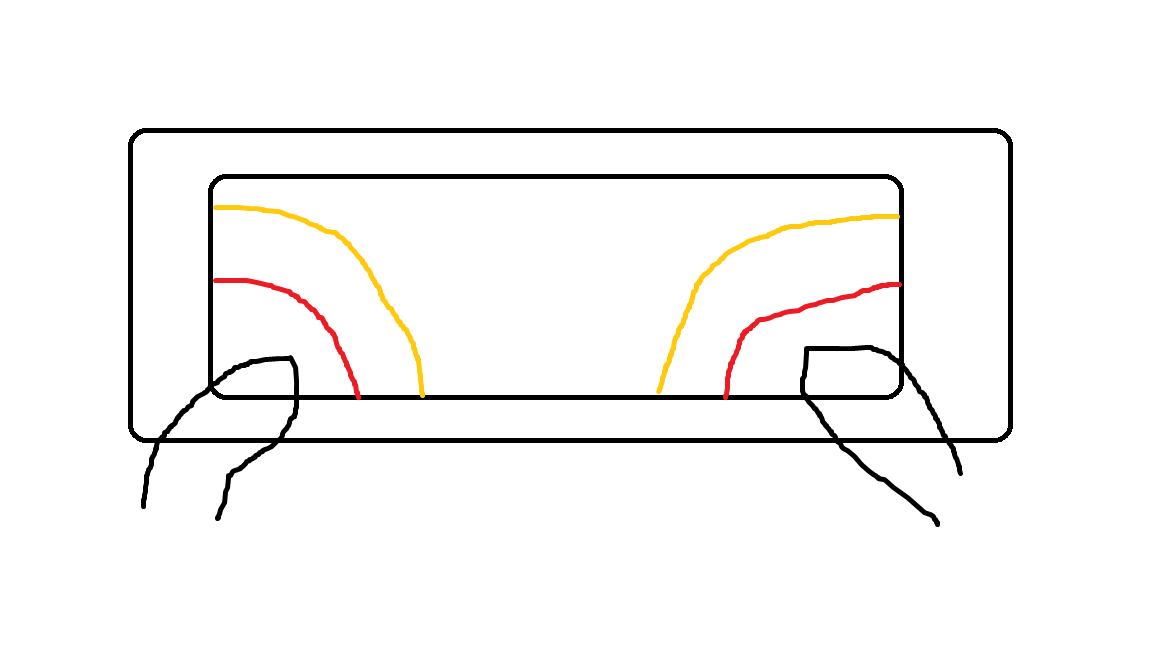
\includegraphics[width=.8\textwidth]{chapters/img/gamerStance.png}

The player keep the phone in landscape position with two thumbs near the bottom corners of the screen. We can easily see that a small part of the screen is easily accessible (Red area), a little bigger area that can be stil accessed (Orange area) and the rest of the screen very hard for interaction.

\paragraph*{Casual player}

The player keeps the device in one hand and uses the secund one to operate on the screen. The hole area of the screen is accessible, but the user cannot touch instantly two distant places.

\paragraph*{Subway player}

The player plays for short time usually in rush. Keeps the phone in one hand controlling it with finger of this hand. This type of player has minimal reach and the control area is very small, additionally  multitouch control method is unacceptable.

This three types of players demand totally different interface for the game. There is no solution that will fit to any two types of the player. During the design stage, the developing team has to decide what type of player they expect. Moreover when we think about contextual games it is possible that the external context will prefer one of these types of interaction for example if player has to run/move with the phone, we have a subway type player, no sophisticated  interaction is possible during movement.

Let us now cover some basic methods of interaction and their implementation in Cordova.

\section{Tap, sigle touch}
This method of interaction have been used in this course all the time. All types of buttons, clickable images represents this simplest control method. However for real fast interaction it is suggested to use touch events instead of click events. The reason is that mobile devices have to spend some time (around 300 milliseconds) to translate native touch event to click one.

\section{Drag, continuous touch}
The mobile devices natively support touch events: touchstart, touchend, touchcancel, touchmove. As for default touch support multitouch, it tracks more than one finger separately. The simple example below presents how touches can be used for simple drawing application.

As usual starting with html file:

\htmlfile{chapters/code_samples/chapter_mobile_game_interface/code1.html}

Now we will build a index.js file. First we have to register event listeners for all touch events.

\begin{js}
var app = {
    initialize: function() {
        document.addEventListener('deviceready', this.onDeviceReady.bind(this), false);
    },

    onDeviceReady: function() {
        var canva = document.getElementById("drawing_canva");
		canva.addEventListener("touchstart", this.onTouchStart.bind(this), false);
		canva.addEventListener("touchend", this.onTouchEnd.bind(this), false);
		canva.addEventListener("touchmove", this.onTouchMove.bind(this), false);		
		this.lastTouch = {x:null, y:null};
		this.colors = ['#aaaaaa', '#ffaaff', '#01ffe3'];
		this.color = 0;
    },
\end{js}

We define three fields that will be used later:
\begin{description}
  \item[lastTouch] - represents coordinates of last registered touch, at this x, and y are null as no touch have been initiated yet,
  \item[colors] - table off colors that will be used, the idea is to change color with the start every new touch,
  \item[color] - the actual color to be used when drawing.
\end{description}

Now the operations connected to specific touch events. Let us start with touchstart:

\begin{js}
    onTouchStart: function(event){
		event.preventDefault();
		console.log("TouchStart");
		var touches = event.changedTouches;
		this.color++;
		if (this.color== this.colors.length) this.color=0;
		this.drawBall(touches[0].pageX, touches[0].pageY);
	},
\end{js}

\begin{explain}
The first line event.preventDefault is a very important one, we do not want the device to process the event further, this could for example result in firing a click event. Next we obtain the information about all touches via event.changedTouches, every touch have properties pageX, pageY that contains coordinates of touched place.
\end{explain}

The drawing of a ball uses a known canvas drawing:

\begin{js}
    drawBall: function(x, y){
		console.log("drawing: ["+x+","+y+"]");
		this.lastTouch.x=x;
		this.lastTouch.y=y;
		var el = document.getElementById("drawing_canva");
		var ctx = el.getContext("2d");
		ctx.beginPath();
		ctx.arc(x, y, 4, 0, 2 * Math.PI, false);
		ctx.fillStyle = this.colors[this.color];
		ctx.fill();
	},
\end{js}

\begin{explain}
Here we record the new x, y as the lastTouch coordinates and draw a circle on this position.
\end{explain}

As we would like to continue drawing while the touch event continues, we do that in touchmove event handler:

\begin{js}
    onTouchMove: function(event){
		event.preventDefault();
		console.log("TouchMove");
		var touches = event.changedTouches;
		this.moveBall(touches[0].pageX, touches[0].pageY);
	},
    moveBall: function(x, y){
		console.log("drawing: ["+x+","+y+"]");
		var el = document.getElementById("drawing_canva");
		var ctx = el.getContext("2d");
		ctx.beginPath();
		ctx.moveTo(this.lastTouch.x, this.lastTouch.y);
		ctx.lineTo(x, y);
		ctx.lineWidth = 4;
		ctx.strokeStyle = this.colors[this.color];
		ctx.stroke();
		this.lastTouch.x=x;
		this.lastTouch.y=y;
	}
\end{js}

\begin{explain}
The drawing when finger is moving, is done using ctx.moveTo and ctx.lineTo methods, after the end of operation we reset the lastTouch coordinates.
\begin{warning}
If we comment the last two lines, the drawing method will be totally different, however, this can be a suggestion how to implement virtual joystick controller.
\end{warning}
\end{explain}

If we run this exiting code we will see that when moves start we draw a circle, after that the lines that follow the movement are drawn. The final result is not symmetric as we can easily see the ball at the beginning of the line and nothing at its end. To repair this we add appropriate touchend handler:

\begin{js}
    onTouchEnd: function(event){
		event.preventDefault();
		console.log("TouchEnd");
		var touches = event.changedTouches;
		this.drawBall(touches[0].pageX, touches[0].pageY);
	},
		
\end{js}

In the presented example we have skipped touchcancel event as not applicable.

\section{Virtual Joy}
One of the nicest control method is virtual joystick. We can distinguish two basic vjoy concepts: stationary vjoy - always on the same place, and dynamical one - appears with touchstart. At first let us cover the stationary one. In this example we will use the ball code from accelerator case.

\htmlfile{chapters/code_samples/chapter_mobile_game_interface/code2.html}

In the html we can notice additional canvas element for our virtual joy, this controller will be placed within the area that the ball is moving.

\jsfile{chapters/code_samples/chapter_mobile_game_interface/Ball.js}

\jsfile{chapters/code_samples/chapter_mobile_game_interface/code2.js}

\begin{explain}
All the javascript code that is connected to ball animation is left unchanged. You can notice that the method update  of the object VJoy handles both events touchstart and touchmove. As expected object VJoy represents the logic for our virtual Joy.
\end{explain}

Now we can discuss the code for  our virtual joy:

\jsfile{chapters/code_samples/chapter_mobile_game_interface/VJoy.js}

%

\begin{explain}
The VJoy object needs information about wrapping canvas, the ball that is to be controlled and scale all that is provided during construction. Additionally we have fields scale, actualPosition and positionOffset that will be used later. Actual position will represent a position of user touch and position offset stores coordinates of left top corner of wrapping, the meaning of scale property will be discussed later.

All the interface drawing is done in drawVJoy methods. The control interface consist of two circles, one in the middle is used to show the center, and the bigger one bounds the area. When player touches the control area an additional blue line will show the movement direction of the ball. At the start of the game when there is no actual position no blue line is shown.

The method update connects the control interface with touches and movement of the ball. We have to take into account that relative position of touch to the middle point of the interface should be used for steering the ball movement. That is why actualPosition is connected to positionOffset and half of wrapping canvas width. Additionally we do not want the size of control interface (canvas width) to have a linear impact on ball velocity, for that reason a scale property was used. After setting the velocity and actual position the vjoy is drawn (line 18).
 \end{explain}

\subsection{Dynamic VJoy}
This time we would like our virtual Joy to appear at the place of touchstart and operate only via moving the finger. There is no many changes we have to add. First we crate a new class file DynamicVJov.js.

\jsfile{chapters/code_samples/chapter_mobile_game_interface/DynamicVJoy.js}

\begin{explain}
The class contains a two new methods touchStart and touchEnd. The first one sets the new position of interface wrapping canvas, shows this wrapping canvas and uses known from previous example VJoy class implementation of update method. The touchEnd method just hide the wrapping canvas.
\end{explain}

\jsfile{chapters/code_samples/chapter_mobile_game_interface/code3.js}

\begin{explain}
The main js file differs by creation od VJoy field (line 12) the new class DynamicVJoy is used instead of VJoy. There are also a new bindings of handler for touchstart and touchend events. Both handlers uses methods of the new derived class DynamicVJoy.
\end{explain}

\htmlfile{chapters/code_samples/chapter_mobile_game_interface/code3.html}

\begin{explain}
In the html file we have only few changes, the firs one is to make vjoy\_canvas invisible at the start (display:none). Additionally in line 20 we add a new file DynamicVJoy.js and in next line a new main .js file is included.
\end{explain}

\section{Catapult type control}

We all know the game angry birds, In that game the control used something like a catapult mechanics, player using continous touch define the velocity vector of bird and a end of touch event start the move of the bird. In our example we will use balls and existing DynamicVJoy, when player touch a ball the VYoy will appear, when player stop touching the ball will start move with appropriate velocity.

Let's start with html file:

\htmlfile{chapters/code_samples/chapter_mobile_game_interface/code4.html}

As we see there are two balls. The files Ball.js, VJoy.js and DynamicVJoy.js are exactly the same as in last example, we have only two new files code4.js and CatapultDVJoy.js.

Now look deeper into the main code4.js file:

\jsfile{chapters/code_samples/chapter_mobile_game_interface/code4.js}

\begin{explain}
In the starting method onDeviceReady we can see initialisation of two Ball objects (ball1 line 13, and ball3 line 18). We have to remember we have two object that represent our ball
\begin{itemize}
\item DOM object connected to html element <img> here represented by variable ball\_img (lines 12, 17) - we can call it visual representative of the real ball.
\item Ball objects represented by variables ball1, ball2 (lines 13, 18) - we can call it logical representative of the real ball.
\end{itemize}
The Ball object already has reference to appropriate DOM one, however while the user will touch the DOM element, the touch event object could have access only to visual representative of our ball. Remembering that javascript is a prototype-based language i.e. at any moment we can add a new field/method to existing object. Therefore we add a new reference logical\_ball to a visual ball representative (line 14, 19).

We can see that each ball have a event listener for touchstart, the rest of listeners are connected to the document object.
\end{explain}

Finally we will analyze the CatapultDVJoy.js:

\jsfile{chapters/code_samples/chapter_mobile_game_interface/CatapultDVJoy.js}

\begin{explain}
As a VJoy appears after touchstart event we have to find what object was touched (using touch.target line 9), and get a reference to a proper Ball object \begin{warning} this.ball = touch.target.logic\_ball\end{warning}. 

The method update is almost the same as in VJoy, class, except here we do not change value of velocity of the controlled ball.

In the method touchEnd we hide our VJoj interface and set the appropriate value controlled ball velocity (lines 32, 33).
\end{explain}

\begin{extercises}
As we can see when the player touch one of the balls the VJoy interface appears at its position, however the ball is still moving away from the VJoy. We could solved that by stopping the time (freezing the game) or stopping the ball. The latter is equivalent to setting velocity of the ball to (0,0) at the moment of the first touch. Please make the appropriate changes to the project.

Additionally, the big circle in the VJoy interface is not needed, Please repair that.
\end{extercises}


\end{document}
